\section{Istruzioni per l'utilizzo}

\subsection{Primo avvio}
\subsubsection{Autenticazione}
\label{sec:autenticazione}
All'avvio verrà mostrata una schermata che servirà ad autenticarsi, nella quale bisognerà inserire nome utente e password del proprio account \gloman{Zextras Drive} (Fig. \ref{fig:Vista del login}). In caso di successo dell'operazione si avvierà il \gloman{software}, altrimenti verrà visualizzato un messaggio di errore e chiesto di reinserire le credenziali (Fig. \ref{fig:errore login}).  \newline
Ai prossimi avvii del software l'account verrà automaticamente caricato, a meno che non venga effettuato il logout (\S{}\ref{sec:profilo}).
\begin{figure}[H]
    \centering
    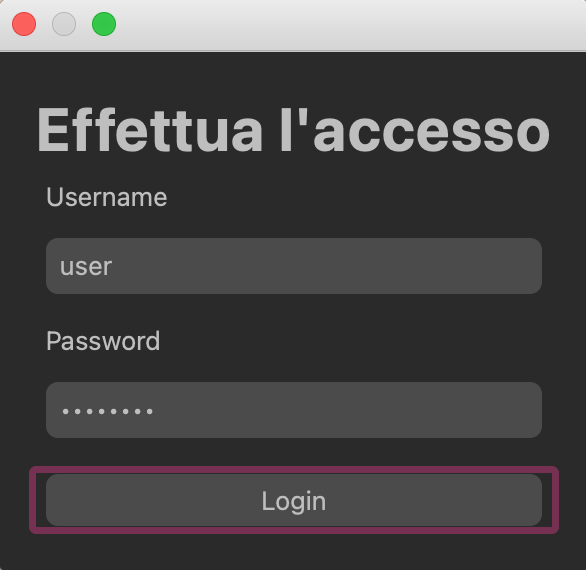
\includegraphics[scale = 0.50]{components/img/login.png}
    \caption{Login}
    \label{fig:Vista del login}
\end{figure}
\begin{figure}[H]
    \centering
    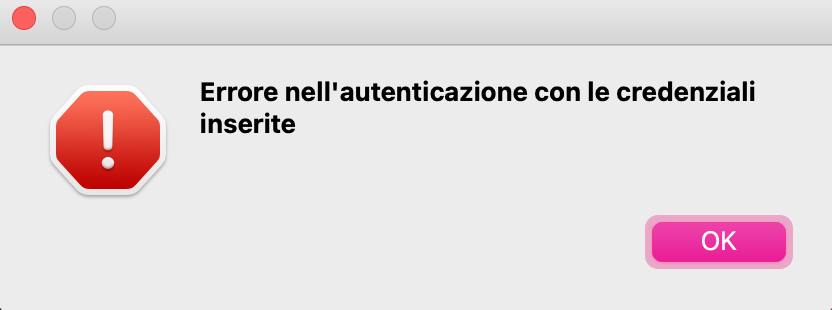
\includegraphics[scale = 0.50]{components/img/err-login.png}
    \caption{Errore di autenticazione}
    \label{fig:errore login}
\end{figure}


\subsubsection{Selezione del percorso da sincronizzare}
\label{sec:selezionepath}
Verrà richiesto di scegliere una cartella nella quale verranno sincronizzati tutti i file. Non si deve scegliere la stessa cartella nella quale è contenuto il programma.
\begin{figure}[H]
    \centering
    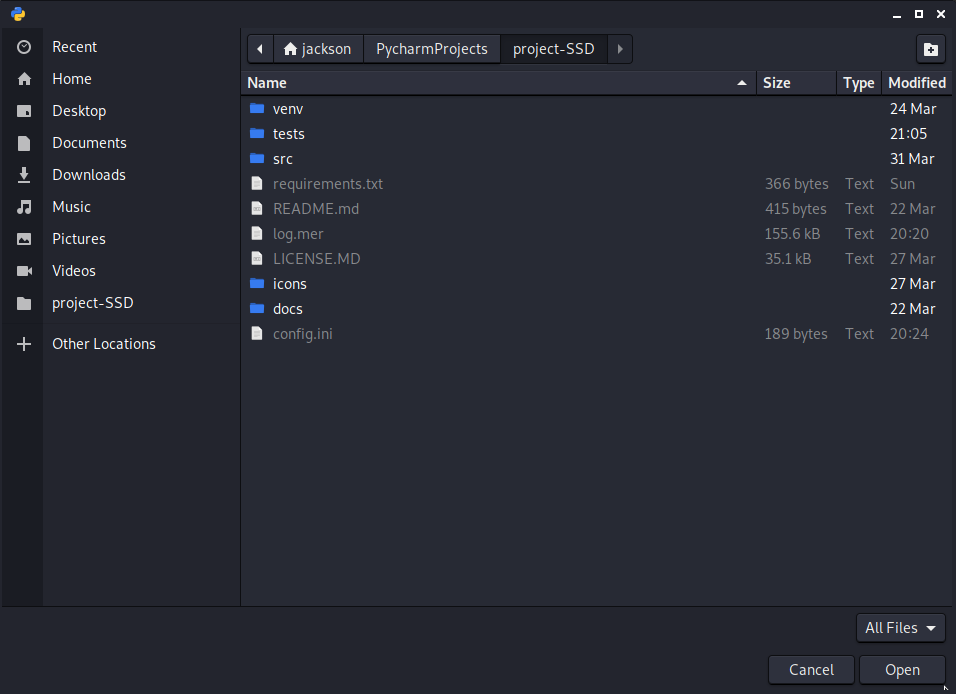
\includegraphics[scale = 0.30]{components/img/selezione-path.png}
    \caption{Selezione del percorso da sincronizzare}
    \label{fig:Selezione del percorso da sincronizzare}
\end{figure}


\subsection{Finestra principale}
\label{sec:principale}
\begin{figure}[H]
    \centering
    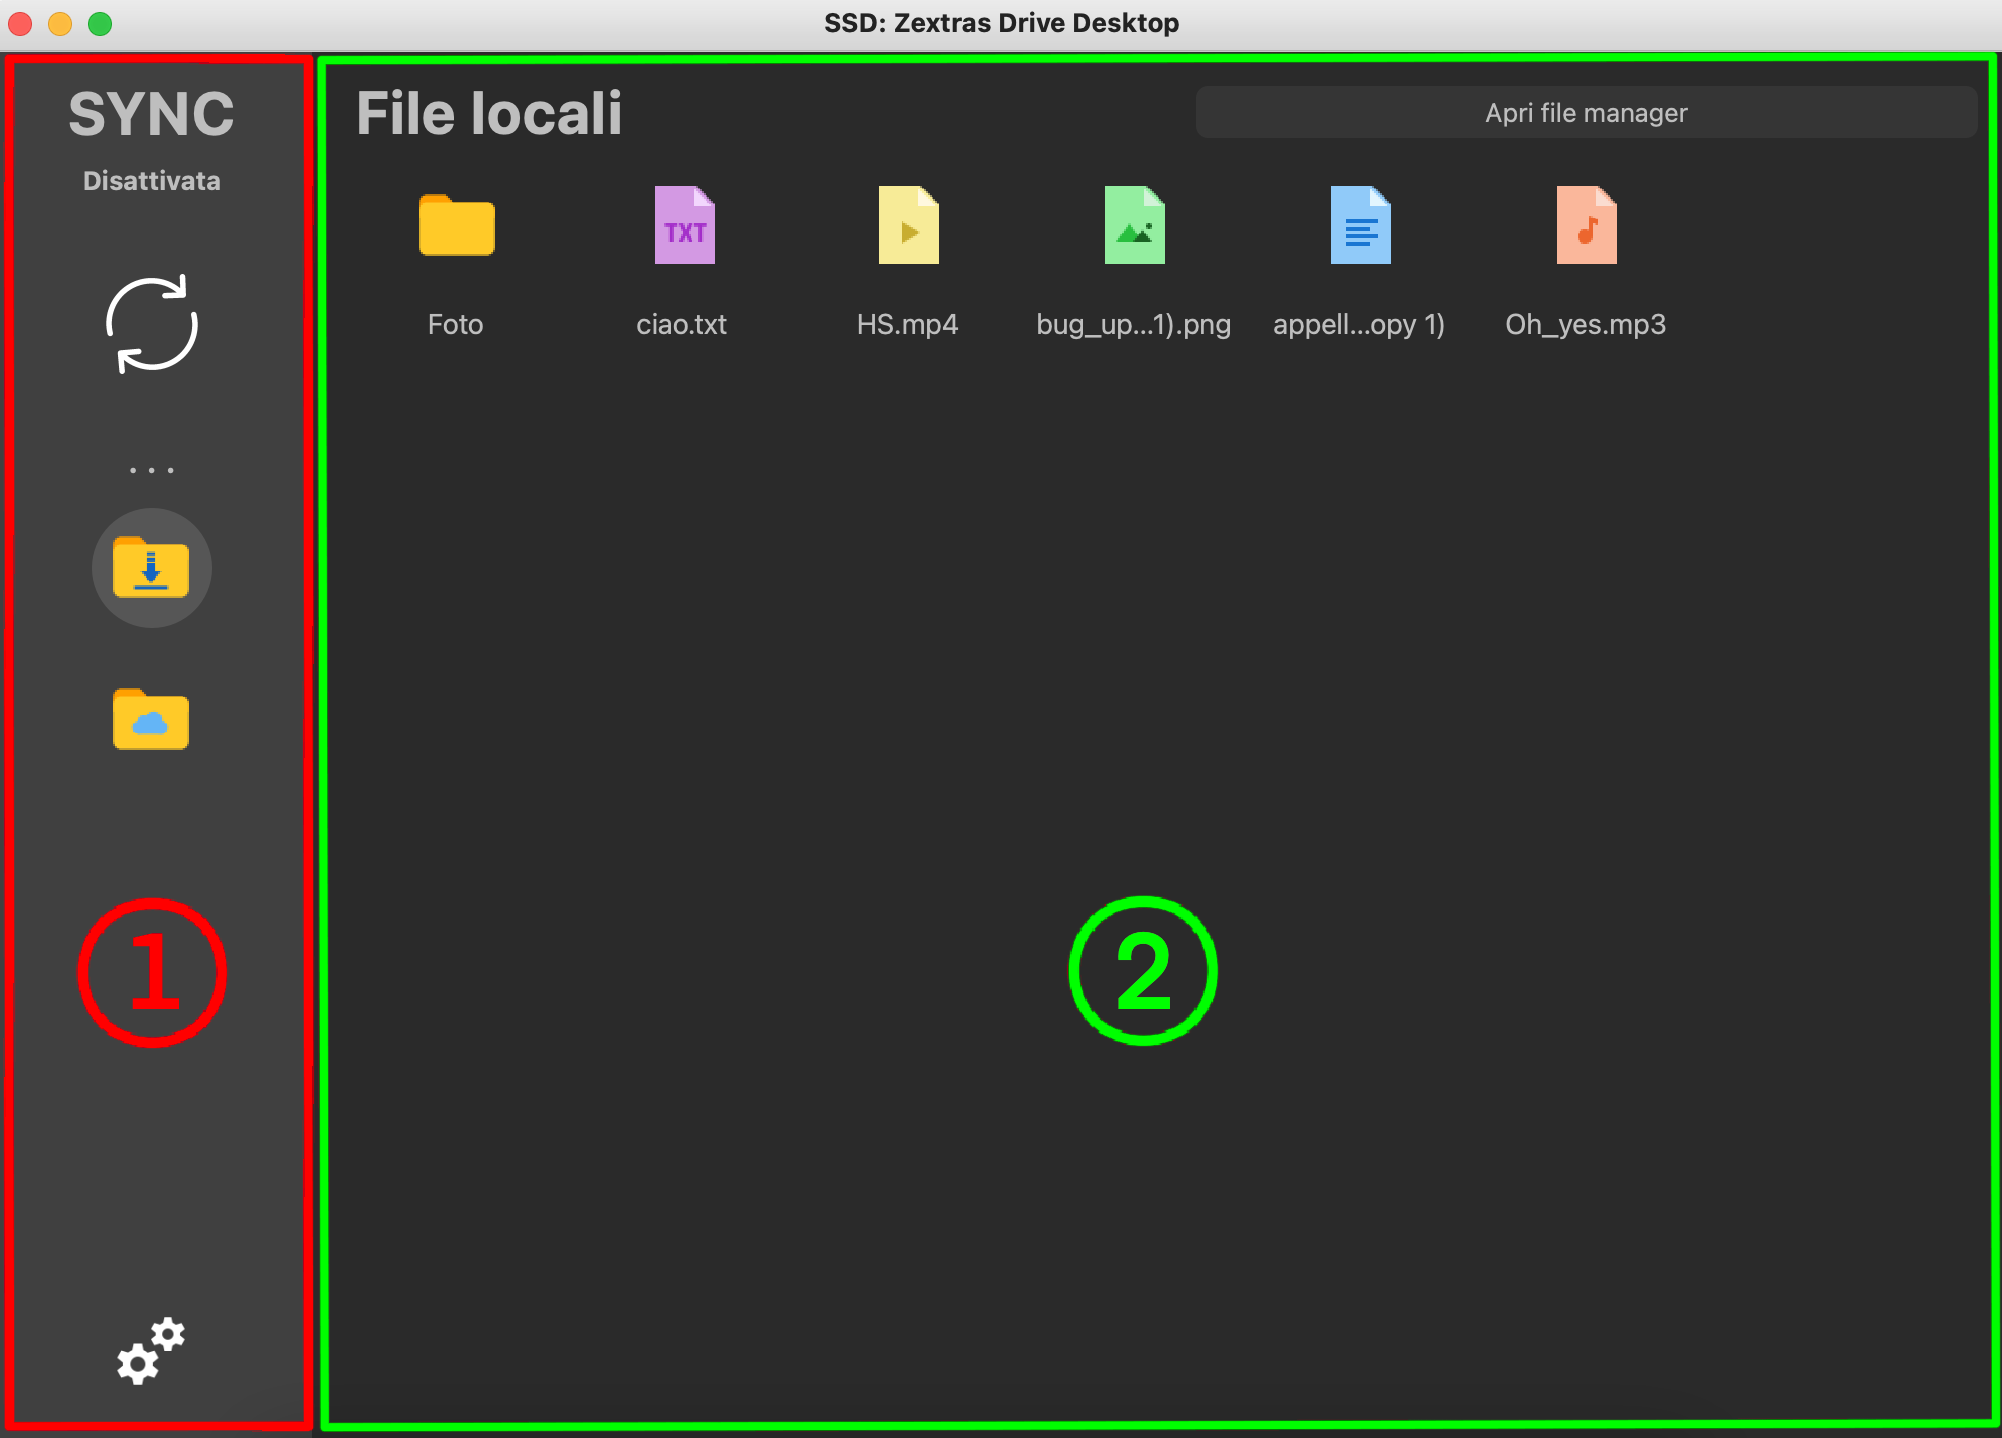
\includegraphics[scale = 0.7]{components/img/Principale.png}
    \caption{Vista schermata principale}
    \label{fig:principale}
\end{figure}
Una volta avviato il software si aprirà una finestra,  mostrata in Fig. \ref{fig:principale}, nella quale verranno visualizzati: 
\begin{enumerate}
\item Menù laterale (\S{}\ref{sec:menu});\
\item Finestra principale, che cambia in base al pulsante selezionato nel menù.\
\end{enumerate}


\subsubsection{Menù laterale}
\label{sec:menu}
Il menù laterale, rappresentato nel punto 1 della Fig. \ref{fig:principale}, è posizionato a sinistra della vista e presenta quattro pulsanti:
\begin{itemize}
\item \textbf{Pulsante di sincronizzazione}: attiva e disattiva la sincronizzazione della cartella locale con il server; \
\end{itemize}
\begin{figure}[H]
\centering
\begin{minipage}[b]{0.45\linewidth}
\centering

\includegraphics[scale=0.5]{components/img/SyncA.png}
\caption{Sincronizzazione attivata}
\label{fig:PsyncA}
\end{minipage}
\quad
\begin{minipage}[b]{0.45\linewidth}
\centering
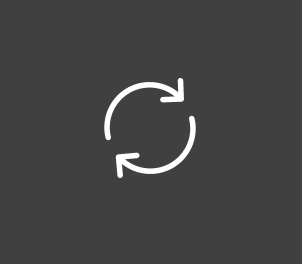
\includegraphics[scale=0.5]{components/img/SyncD.png}
\caption{Sincronizzazione disattivata}
\label{fig:PsyncD}
\end{minipage}
\end{figure}
\begin{itemize}
\item \textbf{Pulsante file sincronizzati}: mostra la cartella locale sincronizzata (\S{}\ref{sec:fileLocali}); \
\end{itemize}
\begin{figure}[H]
    \centering
    
\includegraphics[scale = 1]{components/img/pulsanteFileS.png}
    \caption{Pulsante file sincronizzati}
    \label{fig:PfileSync}
\end{figure}
\begin{itemize}
\item \textbf{Pulsante file remoti}: mostra i file presenti sul server (\S{}\ref{sec:fileRemoti}); \
\end{itemize}
\begin{figure}[H]
    \centering
    
\includegraphics[scale = 1]{components/img/pulsanteFileR.png}
    \caption{Pulsante file remoti}
    \label{fig:PfileRem}
\end{figure}
\begin{itemize}
\item \textbf{Pulsante delle impostazioni}: mostra le impostazioni del software (\S{}\ref{sec:impostazioni}). \
\end{itemize}
\begin{figure}[H]
    \centering
    
\includegraphics[scale = 1]{components/img/pulsanteImpostazioni.png}
    \caption{Pulsante impostazioni}
    \label{fig:PImp}
\end{figure}


\subsection{File locali}
\label{sec:fileLocali}
\begin{figure}[H]
    \centering
    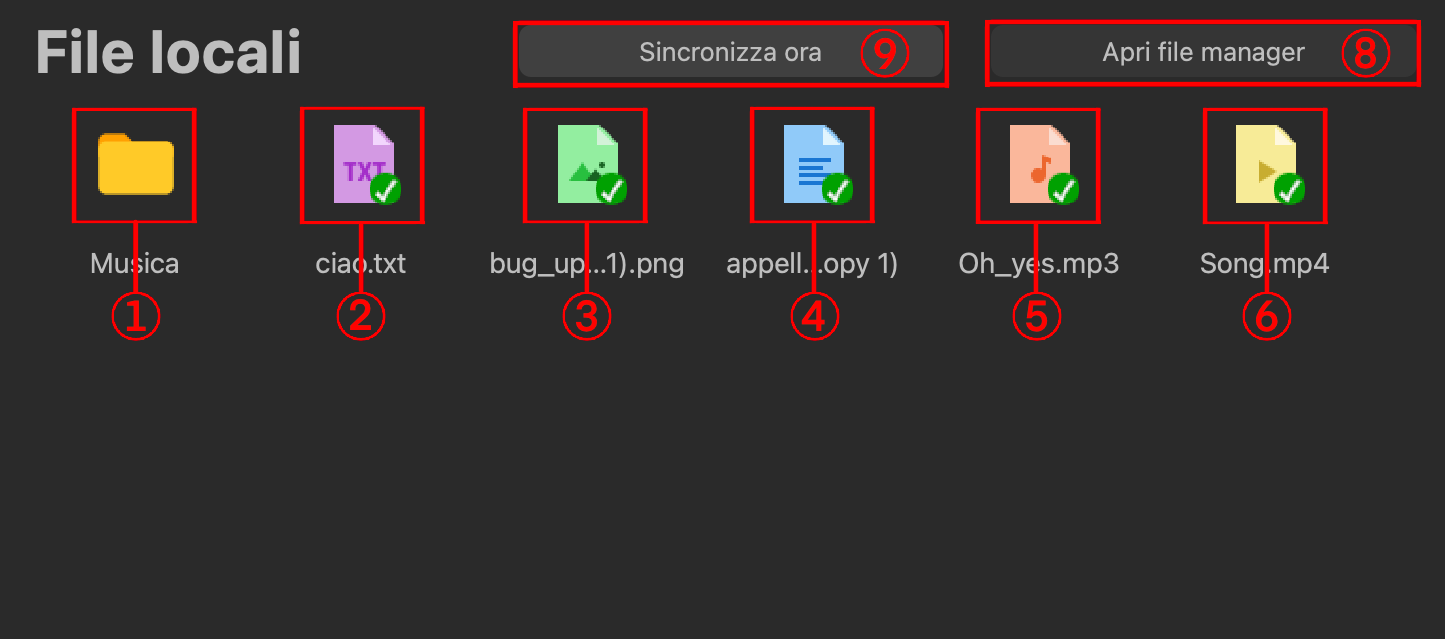
\includegraphics[scale = 0.7]{components/img/fileLocali.png}
    \caption{Vista file locali}
    \label{fig:fileSync}
\end{figure}
La vista si compone di una serie di icone che rappresentano i file o le cartelle presenti nella cartella condivisa. Le icone possono rappresentare:
\begin{itemize}
\item \textbf{Cartella [1]};\
\item \textbf{File di testo [2]};\
\item \textbf{File video [3]};\
\item \textbf{File immagine [4]};\
\item \textbf{File generico [5]};\
\item \textbf{File audio [6]}.\
\end{itemize}
In alto a destra è presente un pulsante [7] che apre la cartella sincronizzata col file manager del computer.


\subsection{File remoti}
\label{sec:fileRemoti}
\begin{figure}[H]
    \centering
    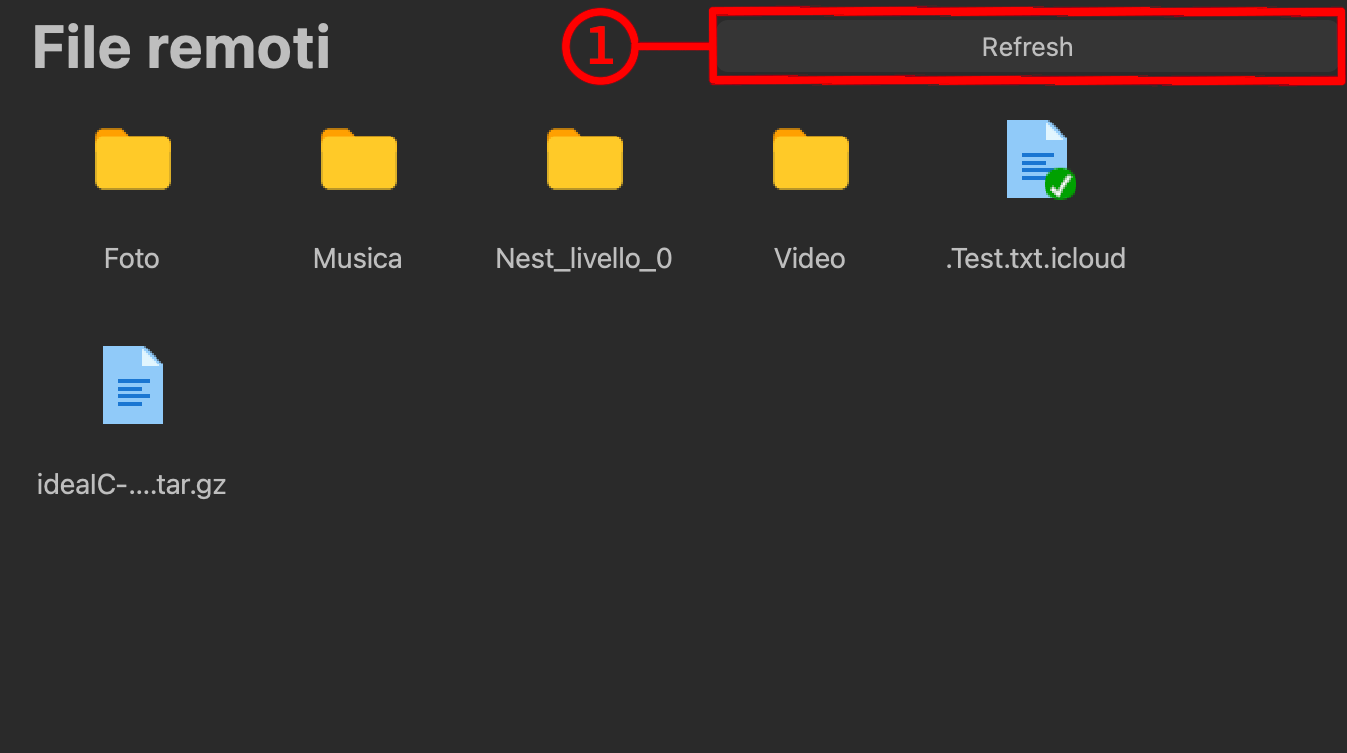
\includegraphics[scale = 0.8]{components/img/fileRem.png}
    \caption{Vista file remoti}
    \label{fig:fileRem}
\end{figure}
La vista si compone di una serie di icone che rappresentano i file o le cartelle presenti nella cartella remota. In alto a destra è presente un pulsante [1] che permette di effettuare il refresh della cartella remota e di sincronizzarla con quella locale.

\subsection{Icone di sincronizzazione}
\label{sec:iconeSync}
\subsubsection{Spunta su sfondo verde}

immagine icona verde\newline

Quando sull'icona del file è presente una spunta su sfondo verde nell'angolo in basso a destra il file è sincronizzato con il server.
\subsubsection{Frecce su sfondo blu}

immagine icona blu\newline

Quando sull'icona del file sono presenti due frecce su sfondo blu il file sta venendo sincronizzato con il server.

\subsubsection{Freccia verso il basso su sfondo blu}

immagine icona blu\newline

Quando sull'icona dei file remoti è presente una freccia su sfondo blu che punta in basso, significa che quel file verrà aggiornato ogni volta che nel server sono presenti delle modifiche.

\subsection{Azioni sui file}
\label{sec:fileActions}

\subsubsection*{Doppio click su un file}
Eseguendo un doppio click su un file nella vista File locali (\ref{sec:fileLocali}) il file verrà aperto dall'applicazione designata dal sistema.
\subsubsection{Click destro su un file}
Eseguendo un click destro su un file nella vista File remoti (\ref{sec:fileRemoti}) è possibile aggiungere o rimuovere un file dalla lista di sincronizzazione.
\subsubsection{Doppio click su una cartella}
Eseguendo un doppio click su di una cartella, sia nella vista File locali che in quella File remoti, si scenderà di un livello, visualizzando il contenuto della cartella selezionata.
\subsubsection{Inserire file nella cartella locale}
Per inserire file nella cartella locale è necessario aprire il file manager utilizzando l'apposito pulsante e aggiungere file da esso.
\subsubsection{Sincronizzare file dal server}
notifica scaricamento file \newline
notifica spazio insufficiente
\subsubsection{Refresh del server}
Per aggiornare la lista dei file visualizzati nella vista \ref{sec:fileRemoti} con le ultime modifiche avvenute nel server bisogna premere il pulsante [1]("refresh").
\subsubsection{Modifica di un file sincronizzato}
La modifica di un file sincronizzato avviene in maniera analoga alla modifica di un qualsiasi file locale, dopo aver effettuato i cambiamenti necessari è sufficiente salvare il documento e questo verrà automaticamente sincronizzato con il server.
\subsubsection{Cancellazione di un file sincronizzato}
L'eliminazione di un file sincronizzato avviene analogamente all'eliminazione di un qualsiasi file locale, dopo aver eliminato il file dalla cartella sincronizzata questa modifica verrà propagata sul server seguendo la politica di sincronizzazione selezionata dall'utente.

\subsection{Impostazioni}
\label{sec:impostazioni}
\begin{figure}[H]
    \centering
    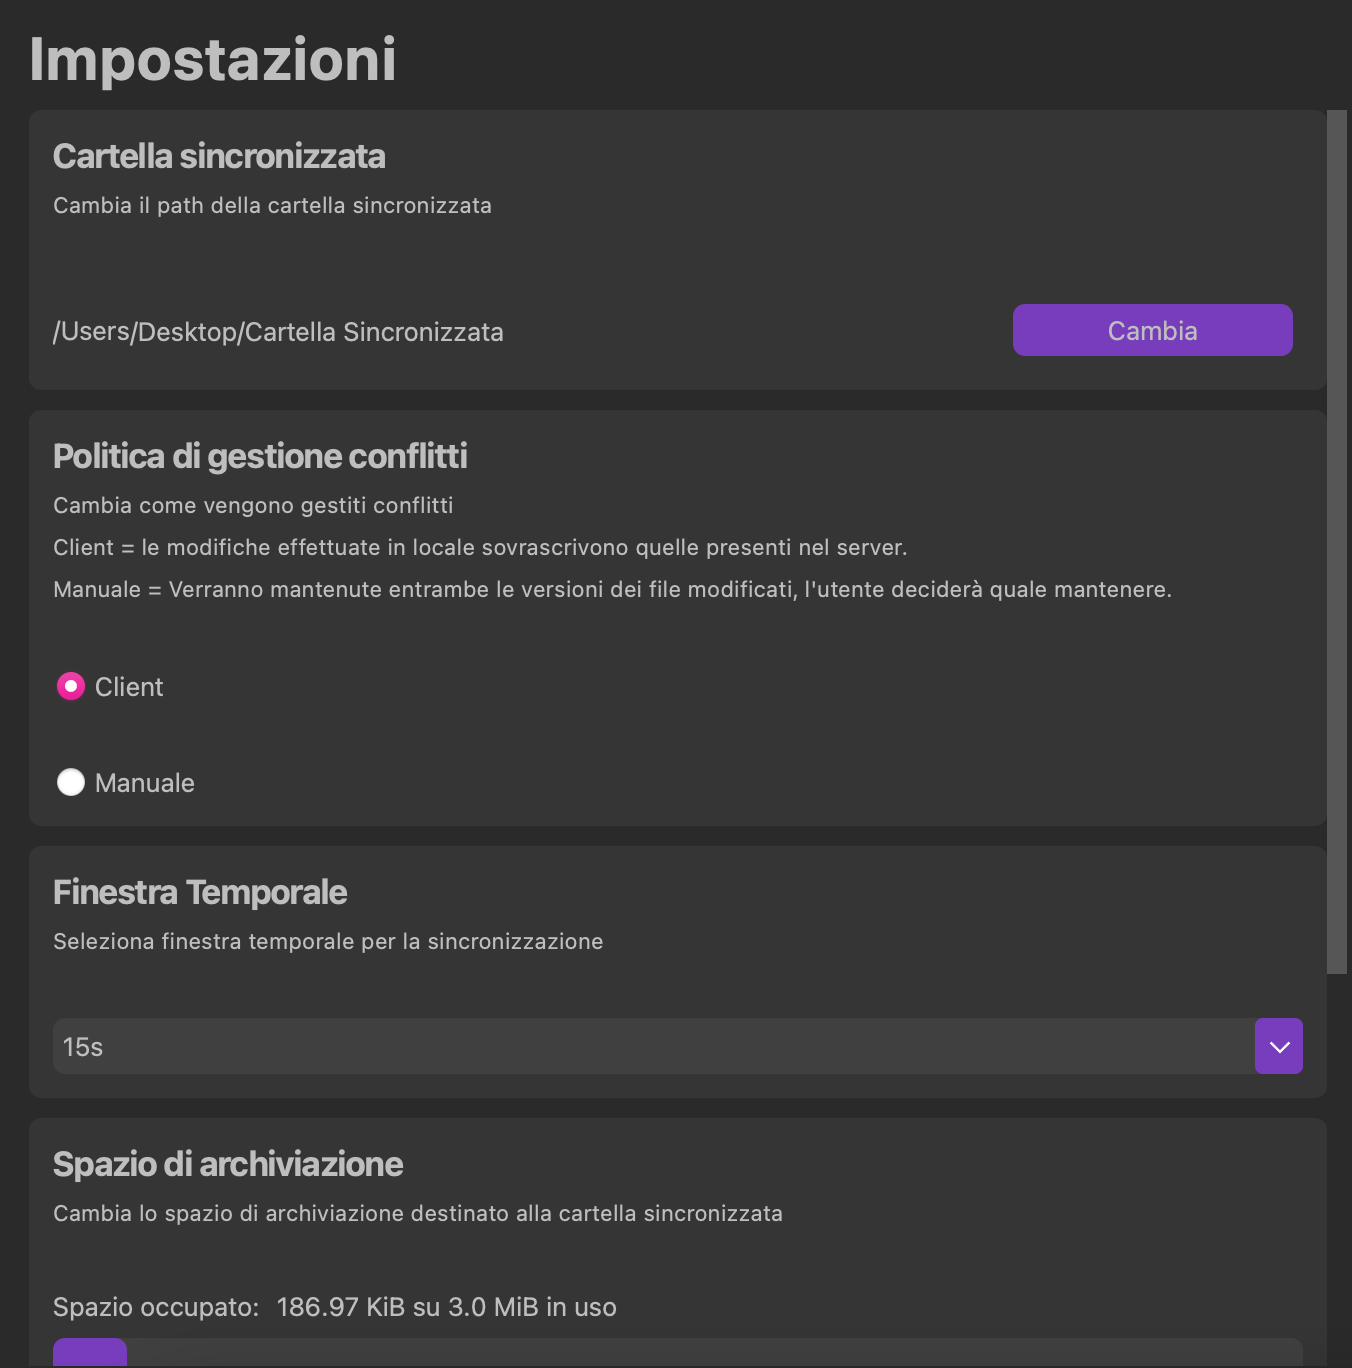
\includegraphics[scale = 0.7]{components/img/vistaImp.png}
    \caption{Vista impostazioni}
    \label{fig:impostazioni}
\end{figure}
La vista mostra una serie di riquadri con i quali è possibile interagire per modificare le impostazioni legate al software. Tramite l'apposita barra posizionata sulla destra è possibile visualizzare l'intera pagina delle impostazioni.

\subsubsection{Modifica path cartella}
\label{sec:cartella}
\begin{figure}[H]
    \centering
    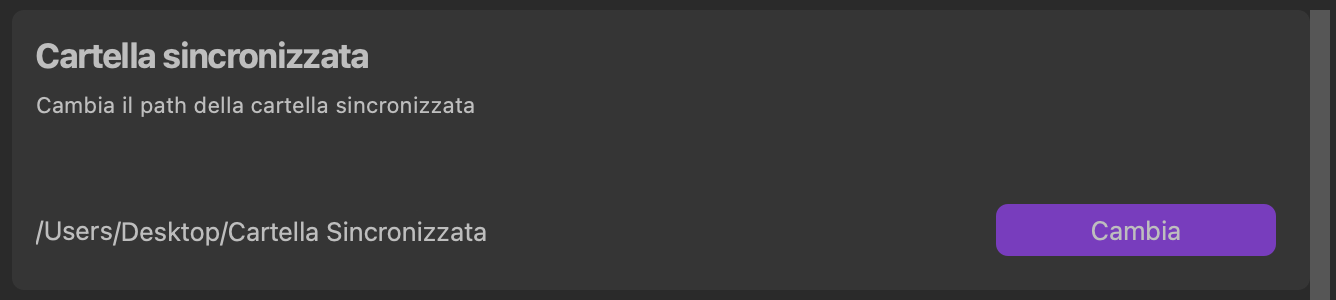
\includegraphics[scale = 1]{components/img/ImpCartella.png}
    \caption{Modifica percorso cartella}
    \label{fig:cartella}
\end{figure}
In questa sezione delle impostazioni è possibile modificare il percorso della cartella sincronizzata. Premendo il pulsante "Cambia" si aprirà una finestra che permetterà di cambiare il percorso (\S{}\ref{sec:selezionepath}).

\subsubsection{Modifica policy}
\label{sec:policy}
\begin{figure}[H]
    \centering
    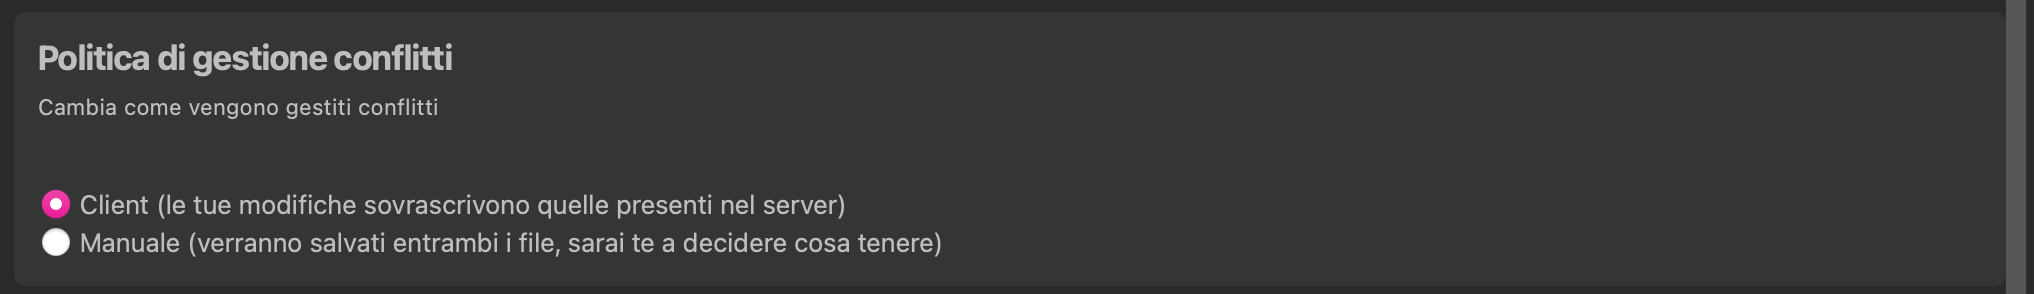
\includegraphics[scale = 0.4]{components/img/ImpPolicy.png}
    \caption{Modifica politica di risoluzione conflitti}
    \label{fig:policy}
\end{figure}
In questa sezione è possibile scegliere la politica di risoluzione dei conflitti. Ci sono due opzioni:
\begin{itemize}
\item\textbf{Client:} selezionando questa opzione le modifiche effettuate in locale andranno a sovrascrivere quelle caricate sul server;\
\item\textbf{Manuale:} selezionando questa opzione, ogni volta che il file in locale differisce dal file presente sul server verranno salvate entrambe le versioni in locale e sarà l'utente a decidere quale mantenere.\
\end{itemize}

\subsubsection{Modifica finestra temporale}
\label{sec:finestra temporale}
\begin{figure}[H]
    \centering
    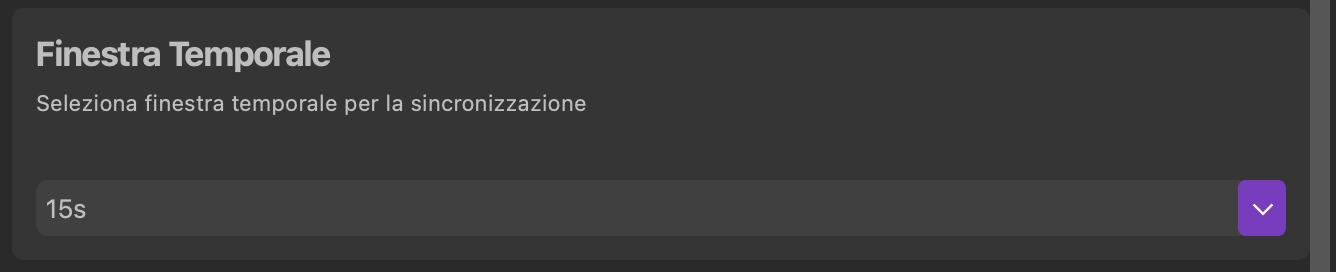
\includegraphics[scale = 0.65]{components/img/ImpFinTempA.png}
    \caption{Modifica finestra temporale}
    \label{fig:finTempA}
\end{figure}
In questa sezione è possibile modificare ogni quanto tempo avviare la sincronizzazione dal server alla cartella condivisa. Cliccando sull'apposita freccia a destra (Fig. \ref{fig:finTempC}) apparirà un elenco di possibili finestre temporali. 
\begin{figure}[H]
    \centering
    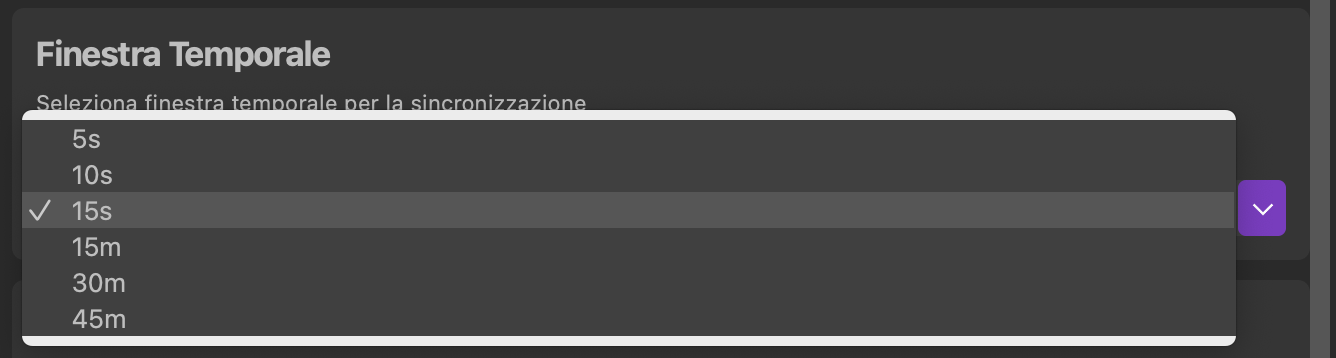
\includegraphics[scale = 0.65]{components/img/ImpFinTempC.png}
    \caption{Vista dopo aver cliccato sulla freccia}
    \label{fig:finTempC}
\end{figure}

\subsubsection{Modifica spazio di archiviazione}
\label{sec:quota}
\begin{figure}[H]
    \centering
    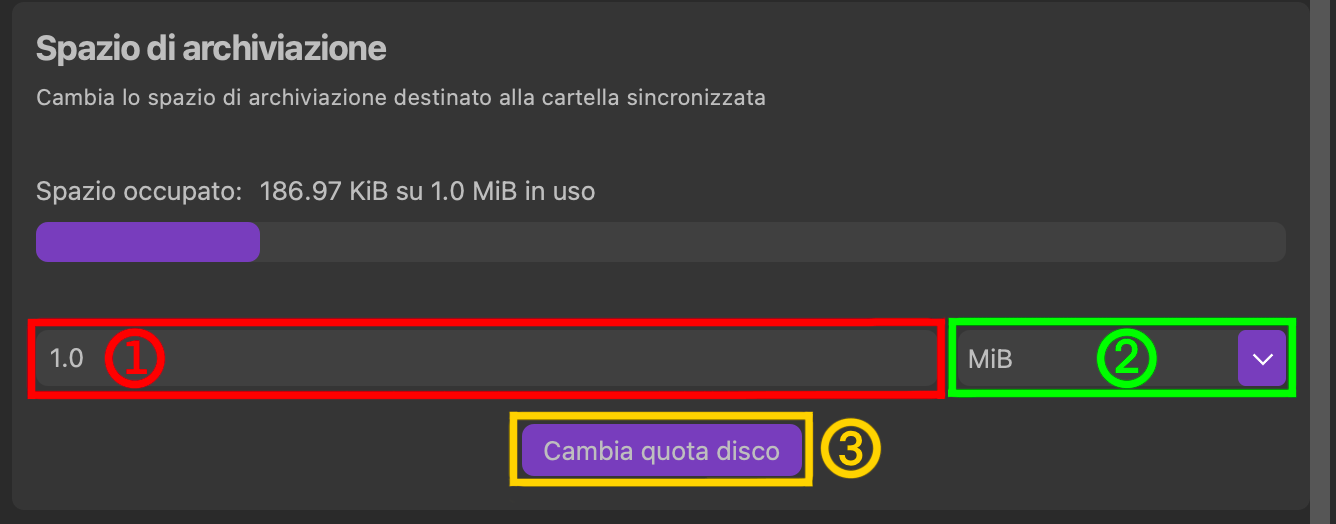
\includegraphics[scale = 0.8]{components/img/ImpQuota.png}
    \caption{Modifica quota disco}
    \label{fig:quota}
\end{figure}
In questa sezione è possibile modificare lo spazio di archiviazione dedicato alla cartella locale. In particolare, seguendo i numeri in Fig. \ref{fig:quota}:
\begin{enumerate}
\item permette di scrivere quanto spazio far occupare alla cartella;\
\item permette di decidere l'estensione del numero scritto (Fig. \ref{fig:quotazoom});\
\item pulsante che modifica lo spazio di archiviazione.\
\end{enumerate}
\begin{figure}[H]
    \centering
    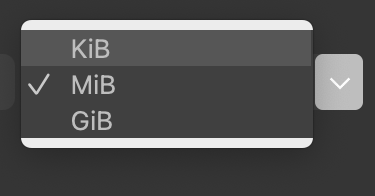
\includegraphics[scale = 1]{components/img/ImpQuota2.png}
    \caption{Vista dopo aver cliccato sulla freccia}
    \label{fig:quotazoom}
\end{figure}


\subsubsection{Profilo}
\label{sec:profilo}
\begin{figure}[H]
    \centering
    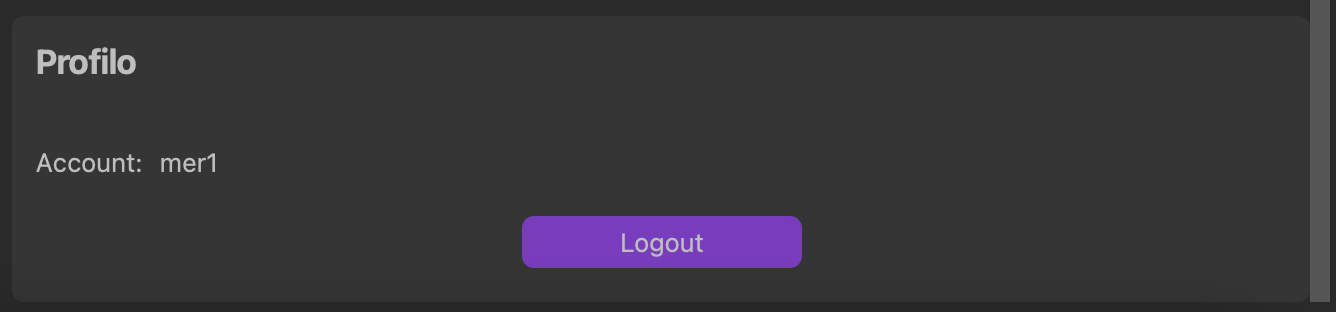
\includegraphics[scale = 0.65]{components/img/ImpLogout.png}
    \caption{Vista logout}
    \label{fig:fileRem}
\end{figure}
In questa sezione è possibile visualizzare il profilo collegato alle credenziali inserite. Inoltre, premendo il pulsante "Logout", è possibile disconnettere il profilo dal software: quest'ultimo si chiuderà e, al prossimo avvio, mostrerà la schermata di login (\S{}\ref{sec:autenticazione})

